\documentclass[border=10pt]{standalone}
\usepackage{tikz}
\begin{document}
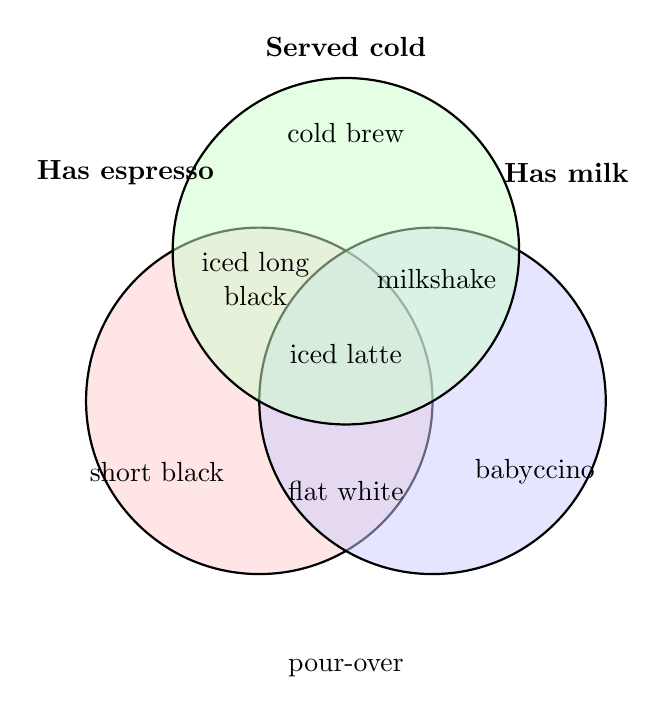
\begin{tikzpicture}
  \def\r{2.2}
  \draw[thick,fill=red!20,fill opacity=0.5] (-1.1,0) circle (\r);
  \draw[thick,fill=blue!20,fill opacity=0.5] (1.1,0) circle (\r);
  \draw[thick,fill=green!20,fill opacity=0.5] (0,1.9) circle (\r);
  \node at (-2.8,2.9) {\textbf{Has espresso}};
  \node at (2.8,2.9) {\textbf{Has milk}};
  \node at (0,4.5) {\textbf{Served cold}};
  \node[align=center] at (-2.4,-0.9) {short black};
  \node[align=center] at (-1.15,1.55) {iced long\\black};
  \node[align=center] at (1.15,1.55) {milkshake};
  \node[align=center] at (0,0.6) {iced latte};
  \node[align=center] at (0,-1.15) {flat white};
  \node[align=center] at (2.4,-0.9) {babyccino};
  \node[align=center] at (0,3.4) {cold brew};
  \node[align=center] at (0,-3.4) {pour-over};
\end{tikzpicture}
\end{document}
